\scanpage{90}

\diagram{\begin{tikzcd}[row sep=large,cells={nodes={anchor=west}}]
\parbox{.88\linewidth}{a) \deleted{\unsure{protore}} \inserted{groupe de t.m.} $T$ sur $Q$, avec $f\in T(Q)$ engendrant $T$ (Zar)} \arrow[d,Leftrightarrow] \\
\parbox{.88\linewidth}{b) Sous-groupe \deleted{de} $M$ de $\overline Q^*$, stable par $\operatorname{Gal}(\overline Q/Q)$} \arrow[d,phantom,"\unsure{\Downarrow|\Updownarrow}"] \\
\parbox{.88\linewidth}{c) Sous-catégorie \unsure{st. pleine} $\mathcal M'$ de la catégorie des vectoriels sur $Q$ avec endomorphisme \inserted{semi-simple} [i.e. de la catégorie des $Q[X]$ modules \inserted{semi-simples} de dim finie sur $Q$] stable par $\otimes$, $\oplus$, sous objet}
\end{tikzcd}}

\deleted{\unsure{a $\Rightarrow$ b}}
Soit donné un groupe de t.m. $T$, avec ``générateur'' $f\in T(Q)$, et soit donné $G_m\xrightarrow{j}T$, ce qui équivaut à se donner $j^*:M\longrightarrow Z$ \inserted{(invariant par $\operatorname{Gal}(\overline Q/Q)$)}, ou une \unsure{graduation} \inserted{\uline{tensorielle}} sur $\mathcal M$.

\inserted{$\varepsilon:T\longrightarrow G_m$ (\deleted{tel que} $\varepsilon\circ j(\lambda)=\lambda^\alpha$), i.e. $j^*(\unsure{\varepsilon^*})=\alpha$.}
\deleted{\unsure{Soit} $\unsure{j(f)}\unsure{=}\unsure{q}$ \unsure{un élément} \unsure{générateur}}
\inserted{i.e. soit donné un objet $\Lambda$ de $\mathcal M$ \unsure{$W\longrightarrow$} \unsure{de rang 1}}
\deleted{i.e. \illegible{3}}
\inserted{i.e. $\Lambda$ de degré $\alpha$.}
\deleted{\unsure{Posons} $\unsure{\varepsilon^*}=q$ \unsure{et} $|\varepsilon(f)|$}
\margin{\figure{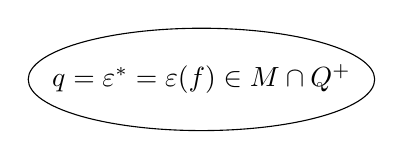
\begin{tikzpicture}\draw (0,0) ellipse (2.2cm and .65cm);\node at (0,0) {$q=\unsure{\varepsilon^*}=\varepsilon(f)\in M\cap Q^+$};\end{tikzpicture}}}

\diagram{\begin{tikzcd}[row sep=large,cells={nodes={anchor=west}}]
\parbox{.88\linewidth}{a) $T^{\unsure{\circ|0}}/\operatorname{Im}j$ est compact.} \arrow[d,Rightarrow] \\
\parbox{.88\linewidth}{b) \inserted{$q>0$ tel} \unsure{que} $\forall\ m\in M$, on a $|m|=\deleted{\unsure{f(f)}}q^{j^*(m)/\alpha}$} \arrow[d,Leftrightarrow] \\
\parbox{.88\linewidth}{c) \inserted{$q>0$ tel} \unsure{que} tout $(E,f)\in\mathcal M$, si $E$ est de degré $i$, les valeurs propres de $f$ dans $E_{\mathbb C}$ sont de val. absolue $q^{i/\alpha}$.}
\end{tikzcd}}

En effet, les valeurs propres de \deleted{$\unsure{E(f)}$ \unsure{et} $f$} $f$, pour $(E,f)\in\mathcal M$ de degré $i$, sont les $m\in M$ avec $\unsure{j(m)}=i$. Donc \deleted{\unsure{b) est plus fort que}} c) et b) sont équivalents.

\deleted{[Ils impliquent a), car $T'=T^{\unsure{\circ|0}}/\operatorname{Im}j$ est un tore \deleted{\unsure{rationnel}} \unsure{possédant} $f'$ ayant la vertu que pour $\forall$ représentation dans un $E$, les valeurs propres de $f'$ opérant sur $E_{\mathbb C}$ sont de val. abs. 1. \unsure{On fera un} \deleted{\unsure{On aura}} \unsure{tore} \unsure{opérant} \inserted{\unsure{semi-simple}} \deleted{\unsure{par des} $\unsure{M^*}$ \unsure{pour} $\unsure{f}$ \unsure{dans} $\operatorname{GL}(E_{\mathbb C})$ \unsure{puis}, \unsure{on le} \unsure{considère} \unsure{opérant} \unsure{sur} $E_{\mathbb C}$ \unsure{et le} \unsure{val. absolue} 1.} Comme $T'_{\mathbb R}$ est un \unsure{sous-groupe} fermé du \unsure{unitaire}, on déduit \unsure{précisément} \illegible{1}]}

\mspage{89}
